\documentclass{article}
\usepackage[utf8]{inputenc}
\usepackage{geometry}
 \geometry{
 a4paper,
 bottom=40mm
 %total={170mm,257mm},
 %left=20mm,
 %top=20mm,
 }
 \title{Cosmological Evidences of Dark Matter through the CMB}
\author{Lorenzo Speri}
\date{}
%\usepackage{hyperref}
\usepackage{natbib}
\usepackage{graphicx}
% ---- Maths -------
\usepackage{amsmath}
\usepackage{amsthm}
\usepackage{physics}
% ---- Links -------
%\usepackage{hyperref}
% citation color
\usepackage[colorlinks=true,citecolor=blue]{hyperref}
% for twnsore
\usepackage{tensind}
\tensordelimiter{:}

% for comments
\usepackage{verbatim}
% wrapping figures
\usepackage{wrapfig}

%  ---- my commands -------
\newcommand{\bea}{\setlength{\jot}{10pt}\begin{eqnarray*}}
\newcommand{\eea}{\end{eqnarray*}}
\newcommand{\beq}{\begin{equation}}
\newcommand{\eeq}{\end{equation}}
\newcommand{\bpsi}{\bar{\psi}}
\newcommand{\dslash}{\slashed{\partial}}
\newcommand{\Dslash}{\slashed{D}}
\newcommand{\Lagr}{\mathcal{L}}
\newcommand{\cpp}{\texttt{C++} } 
\newcommand{\mpi}{\texttt{MPI} } 
\newcommand{\de}{\nu}
\newcommand{\T}{\text{TT}}
\newcommand{\h}{\mathscr{H}}
\newcommand{\ten}{\mathscr{T}}

\begin{document}

\maketitle

\vspace{3cm}
\section{Introduction}
Many astronomical and cosmological observations suggest that, by using the General Theory of Relativity, there is an invisible form of matter that exerts a gravitational pull on baryonic matter. 
In order to explain such observations, scientists have proposed the existence of Dark Matter, a new form of matter that does not interact electromagnetically and, therefore, it appears invisible to us. 
The fundamental nature of Dark Matter is not well understood yet, and whether Dark Matter is truly a new form of matter or the consequence of new laws of gravity is still matter of debate.\\
One of the most compelling evidence for the existence of Dark Matter is given by the analysis of the Cosmic Microwave Background (CMB).\\
The Cosmic Microwave Background is the electromagnetic radiation coming from the hot plasma of the early stages of the Universe.
As the Universe was expanding, it cooled down to a temperature low enough to form stable hydrogen $e^- + p^+  \rightarrow H + \gamma$ (Recombination). 
As the number density of the free electrons dropped with the expansion, the Thomson scattering $e^- + \gamma  \rightarrow e^- + \gamma$ became inefficient and the photons have since streamed freely through the universe in all directions and they are today observed as the Cosmic Microwave Background \citep{LecturesPdf}.\\
The Cosmic Microwave Background appears to us as the best measured Planck spectrum that we know with fluctuations of order $10 ^{-5}$ around the average temperature $T_{CMB} =2.725$ K.
The fluctuations are extremely important because they contain the crucial information about the primordial plasma and its content. 
In fact, during the early stages of the Universe, the photons were interacting with baryonic matter, which in turn was interacting gravitationally with dark matter.
Thus, the observations of the CMB fluctuations are linked to the energy-matter content of our Universe and dark matter.\\
The aim of this paper is to give a short and concise overview of the physics of the CMB and the cosmological evidence of Dark Matter through the analysis of the CMB fluctuations within the $\Lambda$CDM model assumptions.
We are interested in providing few but fundamental tools to understand the importance of the CMB for Dark Matter.\\
We first give an historical overview of the discovery and measurements of the CMB, then we discuss the main assumptions of the $\Lambda$CDM model and the link between the content of our universe and the cosmological model. 
Afterwards, the phenomenology of the hot plasma is explained with a simplified treatment in order to understand the power spectrum of the CMB.
We conclude with the discussion of the CMB temperature power spectrum and the role of dark matter.


%The recent measurements of the Cosmic Microwave Background (CMB) radiation allowed us to infer the presence of Dark Matter in the Universe. In this summary we will explain qualitatively how the presence of Dark Matter influences the CMB anisotropies.
\pagebreak
\section{From the Discovery of the CMB to the Planck Mission}
%
%
%
\begin{figure}
\begin{center}
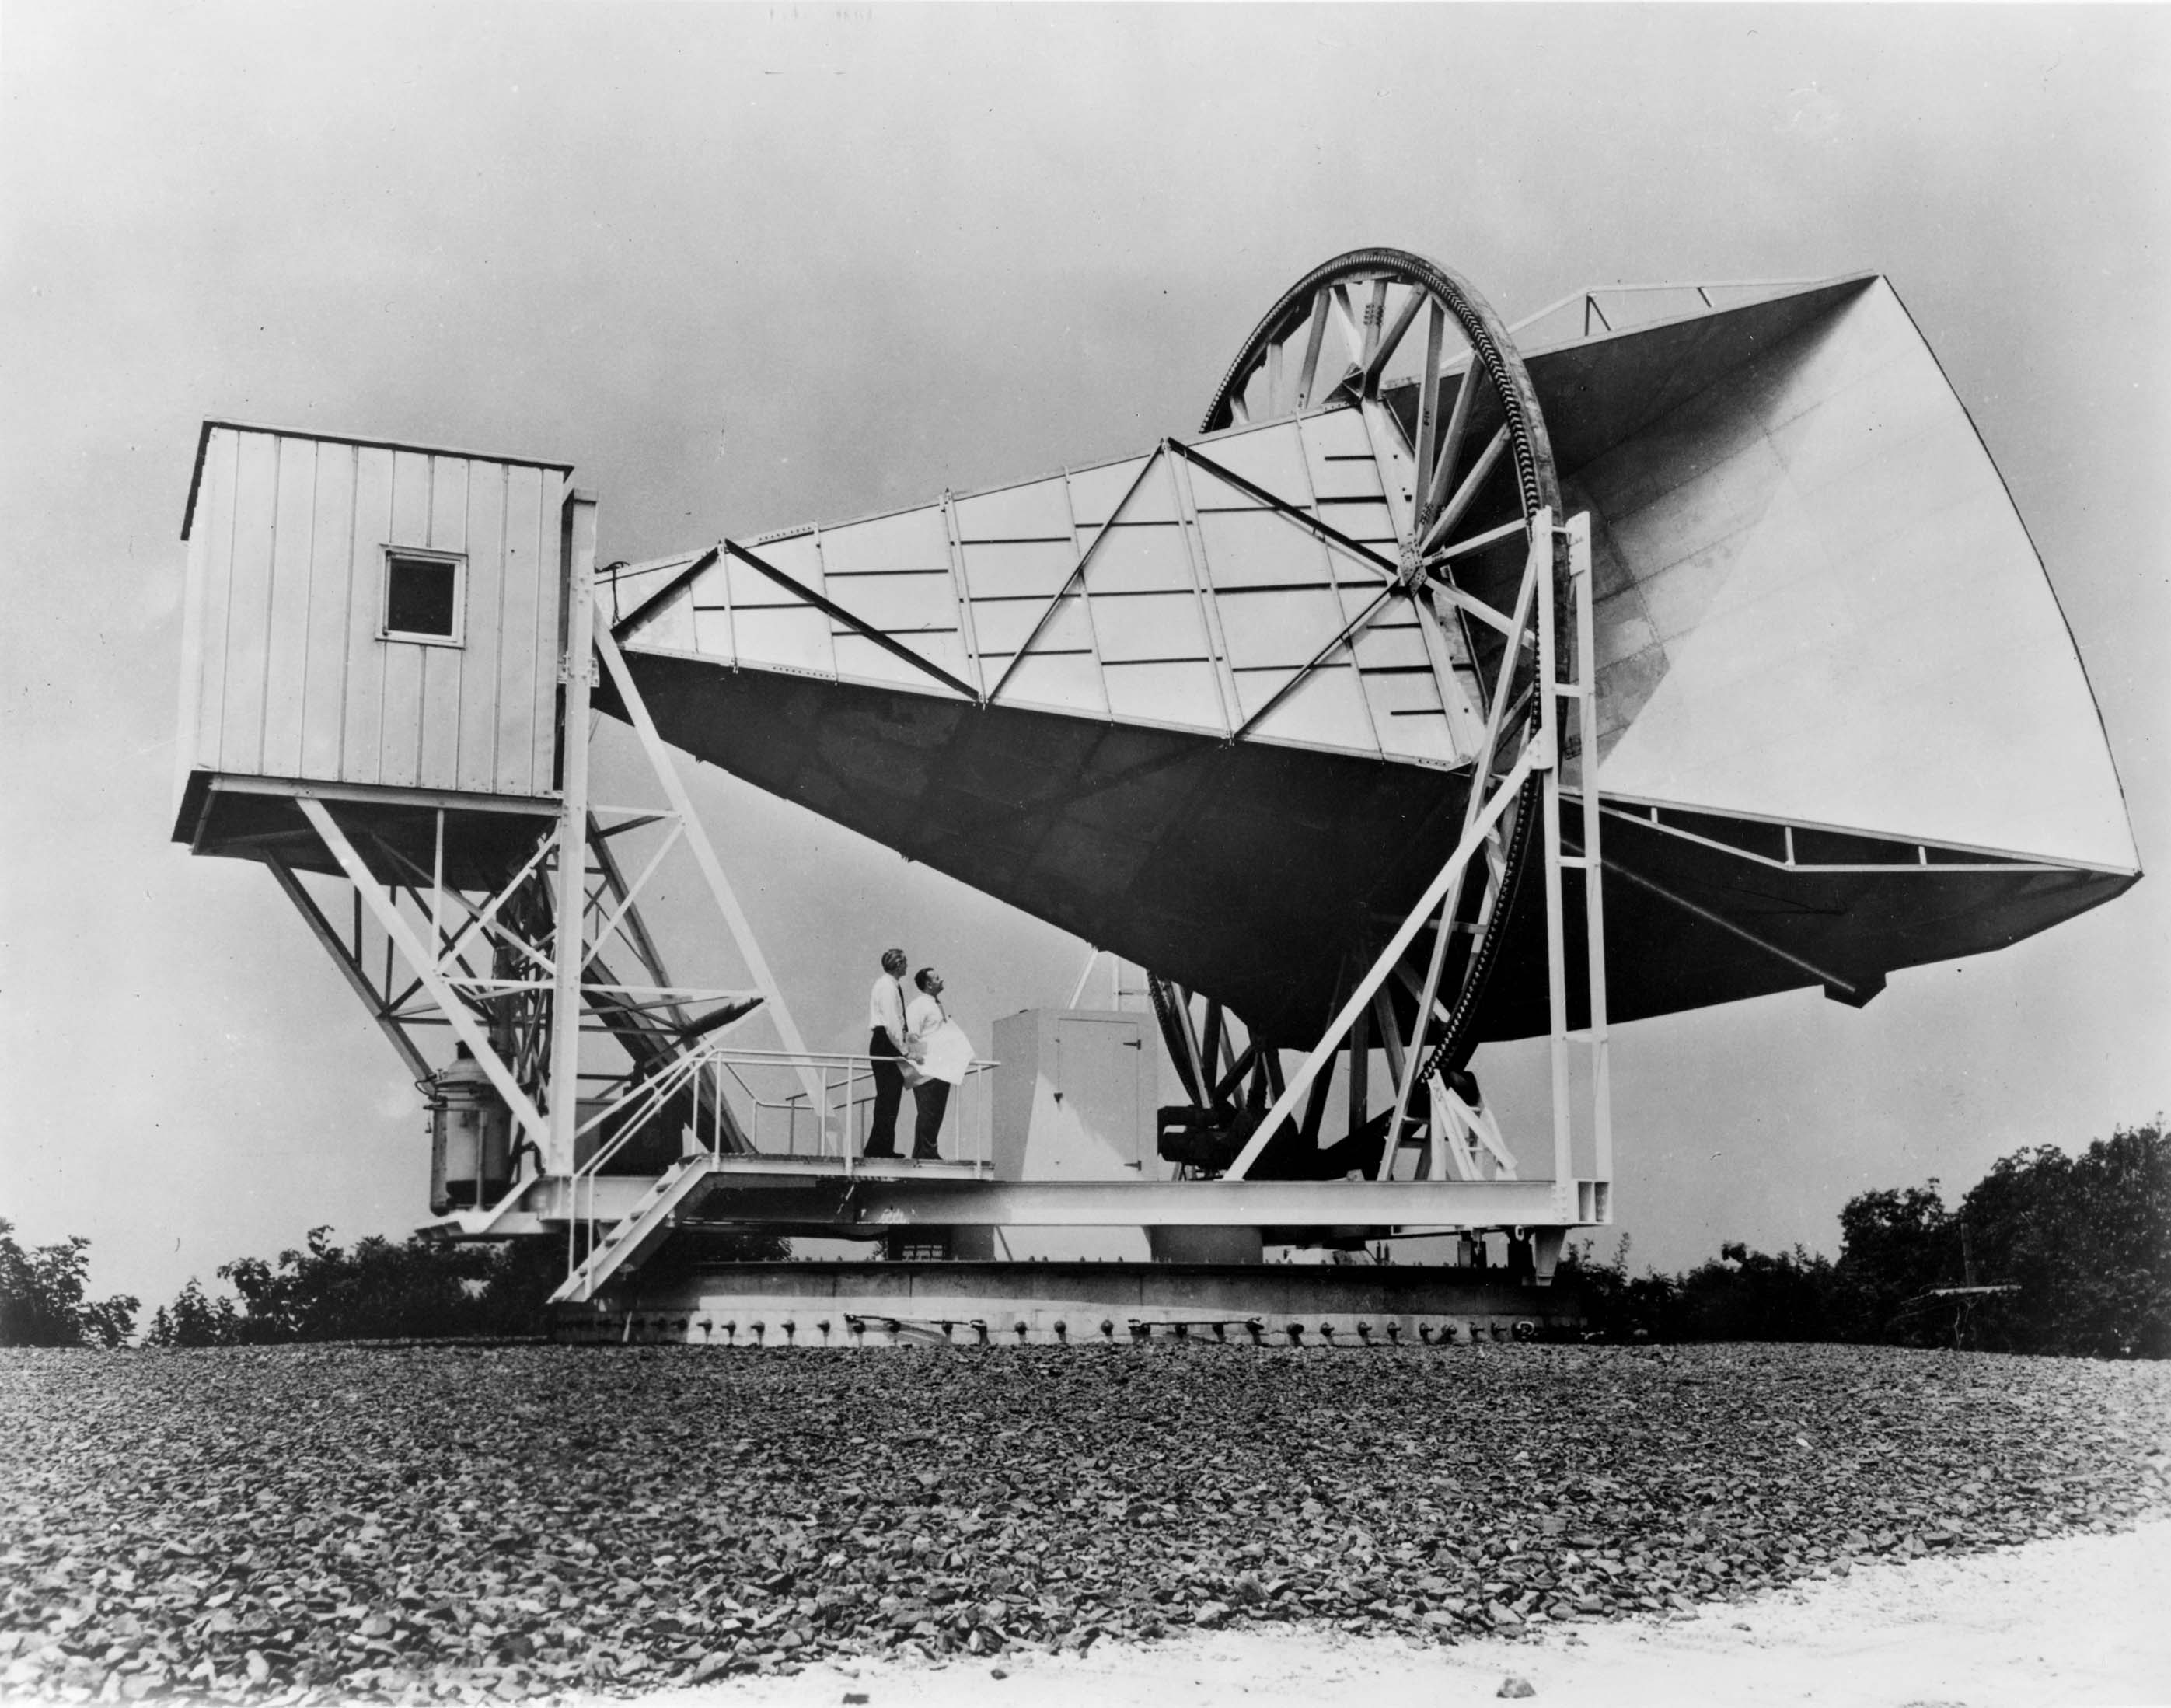
\includegraphics[width=0.7\textwidth]{Horn_Antenna.jpeg}
\caption{The 15 meter Holmdel horn antenna at Bell Telephone Laboratories in Holmdel, New Jersey.
(By NASA - Great Images in NASA Description, Public Domain, \url{https://commons.wikimedia.org/w/index.php?curid=6463768})}
\label{antenna}
\end{center}
\end{figure}
%
%
%
In the 1960s Penzias and Wilson measured an isotropic and constant with time strong signal coming from the sky by using a horn-reflector radio antenna (Figure(\ref{antenna})). 
They tried everything they could do to reduce the “noise” in their system, but the signal remained.\\
In 1965 Arno Penzias and Robert Wilson published the paper: \emph{A measurement of excess antenna temperature at
4080 Mc/s}, where they reported the measurements of an isotropic, unpolarized, and free from seasonal variations excess noise temperature
\citep{penziasMeasurementExcessAntenna1965}.
The explanation of that signal was given by Robert Dicke and his research group at Princeton University: such signal as the relic of an early, hot, dense, and opaque state of the universe\footnote{The existence of the cosmic background radiation had actually been predicted by the physicist George Gamow and his colleagues in 1948} \citep{bucherPhysicsCosmicMicrowave2015}
. \\
The discovery of the CMB created a big excitement and a new era of cosmology began.
Measuring the CMB spectrum and its deviation from the black body spectrum was the new challange.
\\
First of all, the photons of the CMB can be absorbed by the Earth's atmosphere, because the energy per CMB photon (approximately $\sim 6 \times 10 ^{-4}$ eV) is comparable to the energy of vibration or rotation for a small molecule (of water for instance). 
In fact, microwaves with wavelengths shorter than $\lambda \sim 3$ cm are strongly absorbed by water molecules \citep{RydenIntroCosmoPdf}.
This problem could be overcomed by observing the CMB in different bands and from locations where the atmospheric humidity is low, at high altitudes and at low temperatures.
However, the best way to meseaure the CMB spectrum is to use satellites.\\
The first sattellite that was launched to observe the CMB was COBE. 
It did provide a convincing first detection of the CMB anisotropy, and it played a crucial role in determining the viability of the different cosmological models at that time.
\\
After that, WMAP and PLanck space missions  increased the accuracy of the measurements Figure (\ref{cobe_wmap_planck}).\\
The COBE, WMAP and Planck missions measured the CMB anisotropies with increasing accuracy. COBE, the first CMB satellite, measured fluctuations to scales of 7$^\circ$. WMAP was able to measure resolutions down to 0.3$^\circ$ in five different frequency bands, with Planck measuring all the way down to just 5 arcminutes (0.07$^\circ$) in nine different frequency bands in total.\\
Nevertheless the satellites improved their accuracy, many other sources of noise were encountered such as the light coming from the center of our galaxy, other stars and other objects in the universe, in addition to the relative motion of the satellite with respect to the CMB (Figure (\ref{cobe_map})).\\ 
Finally, observations and statistical analysis showed that the CMB spectrum is close to a black body spectrum up to fluctuations of order of $10^{-5}$ K (Figure (\ref{cobe_blackbody})).\\
% maybe last sentence in the introduction with the image

\begin{figure}[h]
\centering
    \textbf{Cosmic Microwave Background  Spectrum}\par\medskip
\centering
   {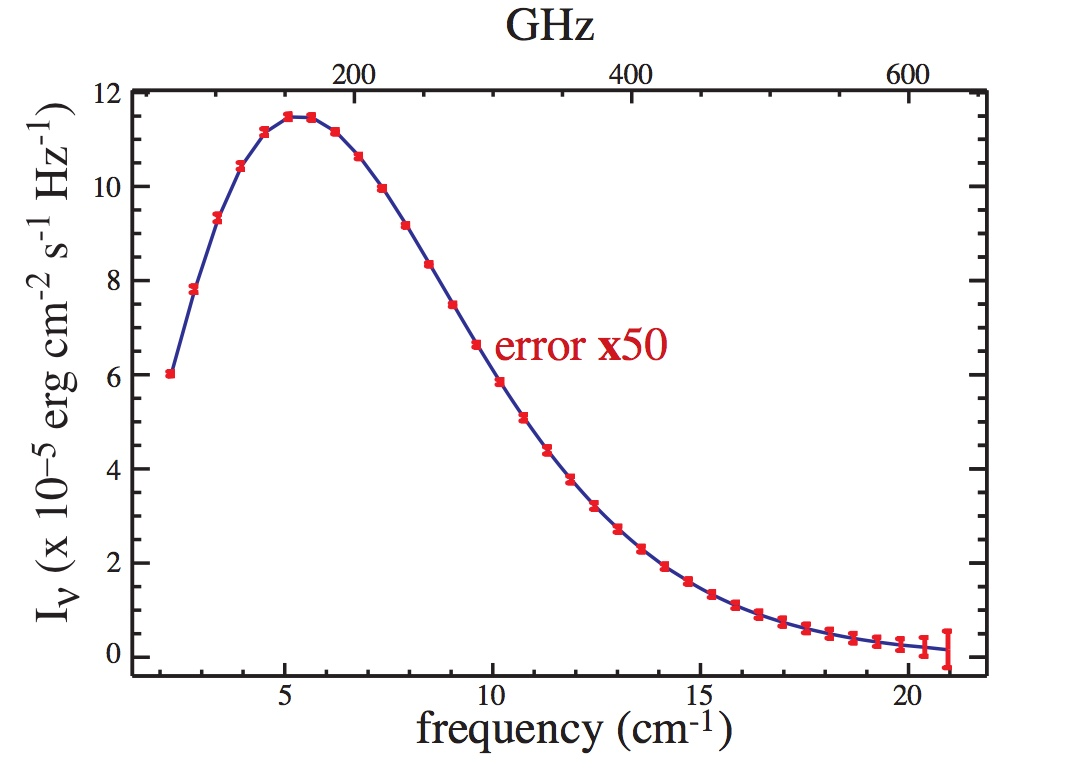
\includegraphics[height=7cm]{blackbody}}
\caption{}
\label{cobe_blackbody}
\end{figure}


\begin{figure}[h]
\centering
    \textbf{The Cosmic Microwave Background anisotropies measured by COBE, WMAP and Planck}\par\medskip
\centering
   {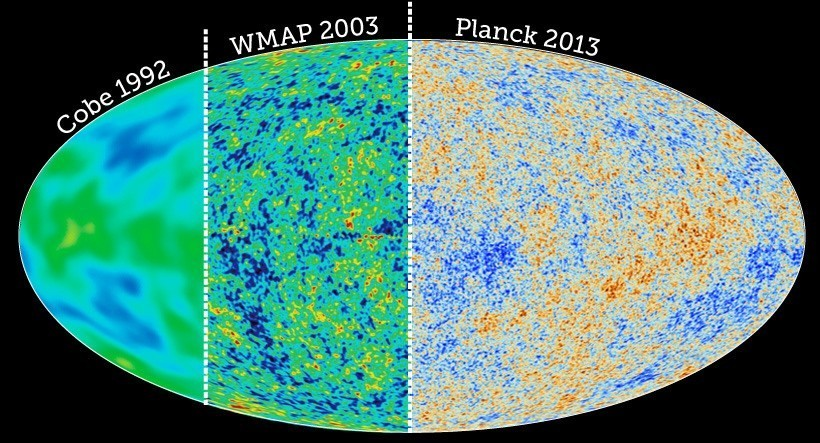
\includegraphics[width=.65\textwidth]{cmb1.jpg}}


\caption{(NASA/COBE/DMR; NASA/WMAP SCIENCE TEAM; ESA AND THE PLANCK COLLABORATION)}
\label{cobe_wmap_planck}
\end{figure}


\begin{figure}
\centering
    \textbf{The CMB sky measured by COBE}\par\medskip
\centering
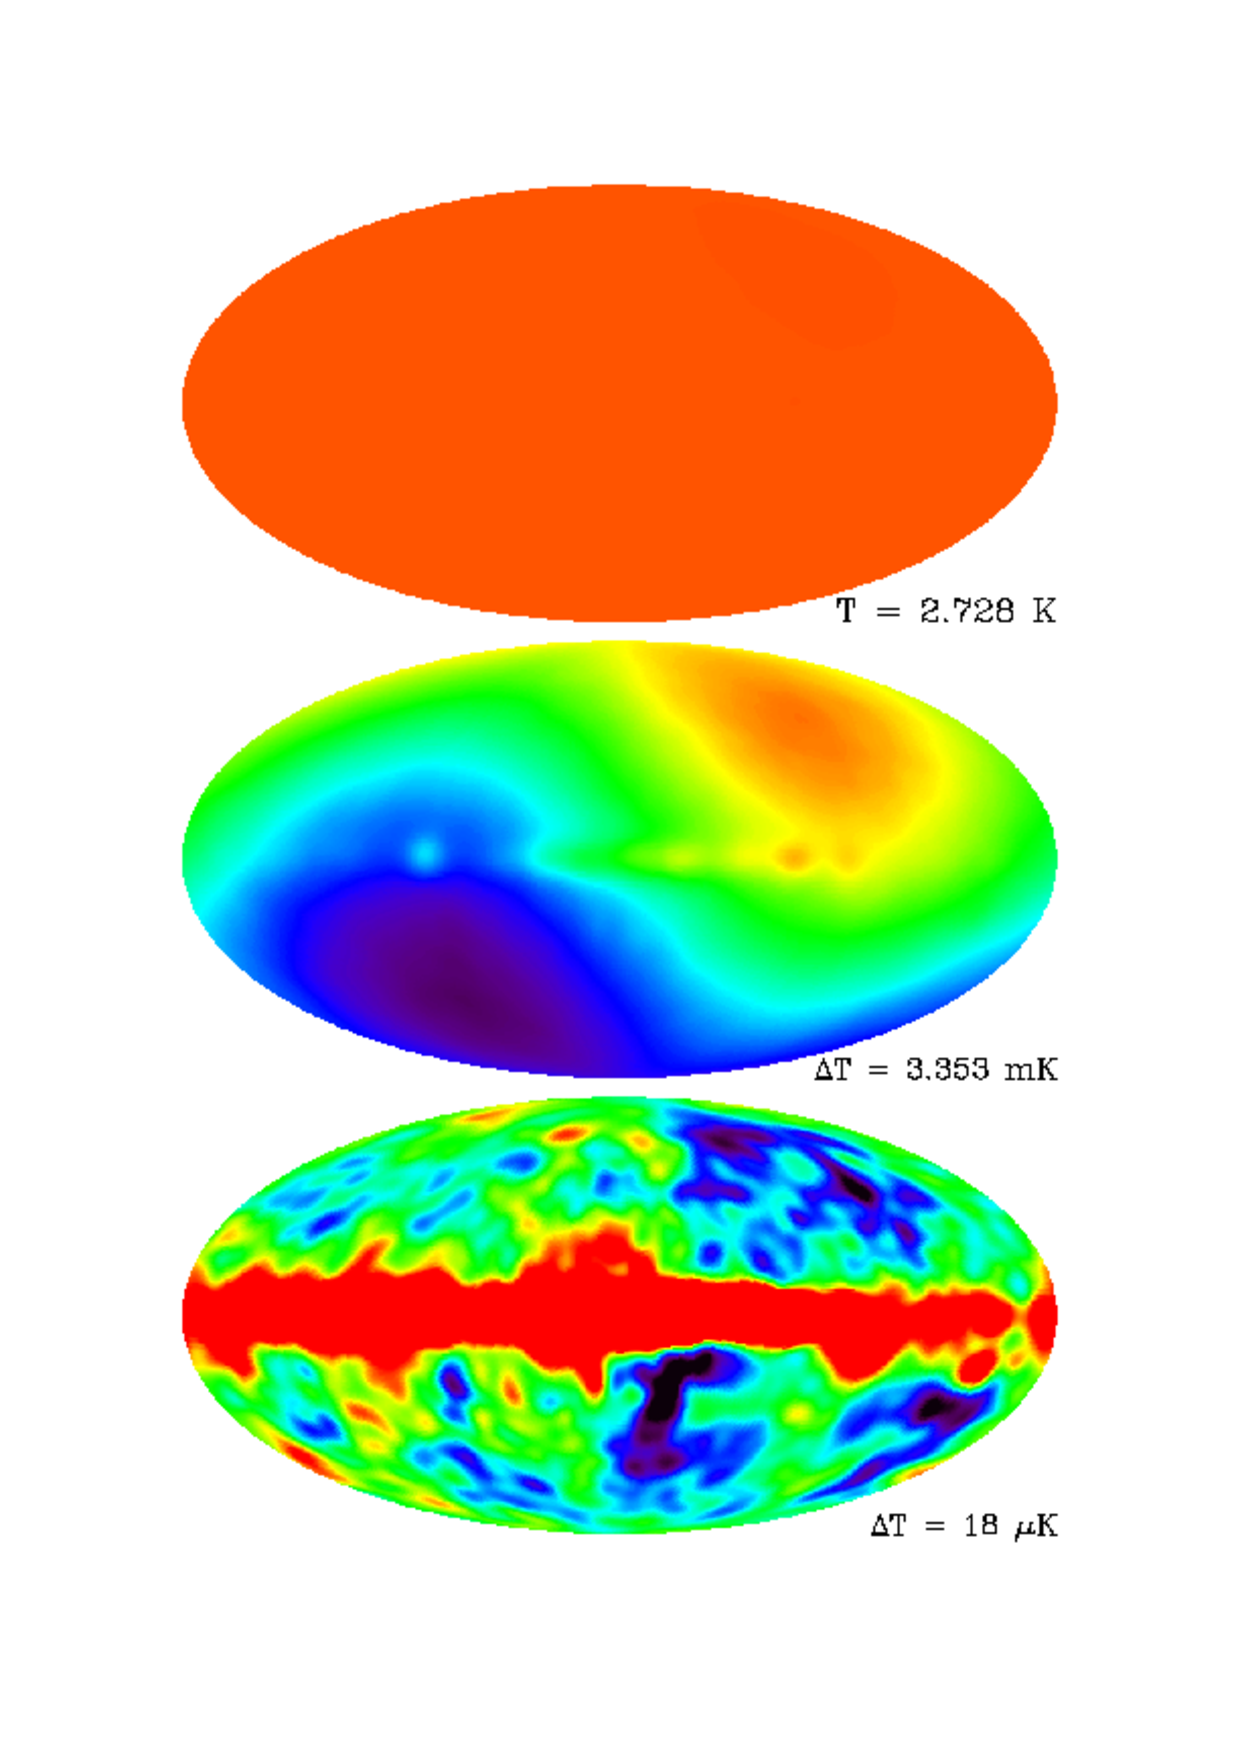
\includegraphics[scale =0.3]{mono_di_cobe}
\caption{The microwave sky as seen by the COBE DMR (differential microwave radiometer) instrument. The top panel shows the microwave sky as seen on a linear tem- perature scale including zero. No anisotropies are visible in this image, because the CMB monopole at 2.725K dominates. In the middle panel, the monopole component has been subtracted. Apart from some slight contamination from the galaxy near the equator (corre- sponding to the plane of our Galaxy), one sees only a nearly perfect dipole pattern, owing to our peculiar motion with respect to the rest frame defined by the CMB. In the bottom panel, both the monopole and dipole components have been removed. Except for the galactic contamination around the equator, one sees the cosmic microwave background anisotropy along with some noise. (Credit: NASA/COBE Science Team)}
\label{cobe_map}
\end{figure}

\newpage


\section{Energy-Matter Content of the Universe} 
It is often said that our Universe is made up of $68.8$\% of Dark Energy, and $26.8 $\% by Dark Matter and $4.9 $\% of ordinary matter, but what do we really mean by that?\\
In this section we explain the meaning of these parameters and what is Universe made up of. 
The assumptions and the theoretical framework that we are going to explain will be then used to analyze the observations of the CMB.\\
We assume that the observable properties of the Universe are isotropic and there is not a preferred direction. 
Therefore, the Universe is assumed to be homogenous and isotropic at enough large scales $> 100$ Mpc, at least up to the observable universe.\\
Another important assumption is that there exists a class of observers at rest with respect to the Cosmic Microwave Background \citep{bartelmannStandardModelCosmology}.
Let us clarify this concept.
The CMB appears as an homogeneous map at temperature $T=2.7$ K as shown in the first panel of Figure(\ref{cobe_map}).
After subtracting the average temperature of the CMB from its spectrum, a moving observer with respect with the CMB will see a dipole pattern, where the blue-shifted photons come from the direction the observer is moving toward to and the red-shifted photons from the opposite direction.
Since Earth is not at rest with respect to the CMB, the satellite COBE measured the dipole pattern showed in the second panel in Figure (\ref{cobe_map}).\\
In addition we assume that space-time is described by a metric theory of gravity, and we treat space-time as a 4-dimensional manifold characterized by the metric tensor $g_{\mu \nu}$.
The most general metric $g_{\mu \nu}$ satisfying homogeneity and isotropy assumptions is the Friedmann – Lemaître – Robertson – Walker (FLRW) metric written here in terms of the invariant geodesic distance $\dd s ^2 = g_{\mu \nu} \dd x^{\mu} \dd x^{\nu}$:
\begin{equation}
\label{metric}
\dd s ^2 = -c ^2 \dd t^2 + a^2 (t) \qty( \frac{1}{1-k \, r^2} \dd r^2 + r^2 \dd \Omega ^2 )  
\end{equation}
where $k$ is the space curvature and it determines the geometry of the spatial dimensions, elliptical, Euclidean or hyperbolic for $k>0$, $k=0$ or $k<0$.
The space curvature determines in which kind of three dimensional space we live in and how angles are measured.\\
The scale factor $a(t)$ determines how the distances scale with the evolution of the Universe.
The propagation condition of light is $ds^2 =0$, which implies that the light with frequency $\nu$ and the wavelength $\lambda$ is red- or blueshifted by the same amount as space expands or shrinks:
\begin{equation}
\dfrac{\nu_{emitted}}{\nu_{observed}} = \dfrac{\lambda_{emitted}}{\lambda_{observed}} = 1 + \dfrac{\lambda_{emitted}-\lambda_{observed}}{\lambda_{observed}}=1+z= \dfrac{a(t_{emitted})}{a(t_{observed})}
\end{equation}
\\
Notice that the FLRW metric has $g_{0 i}=0$ due to the isotropy and the two parameters $a(t)$ and $k$ are the only allowed to preserve our assumptions, all the others parameter that we can introduce can be absorbed in these two.
\\ % comments on the redshift, metric, what spatially flat means
If we assume the correctnes of the General Theory of Relativity, we can use the Einstein's field equations
\begin{equation}
\label{einstein_eq}
R_{\mu \nu} - \dfrac{1}{2} R \, g _{\mu \nu} + \Lambda g_{\mu \nu}= \dfrac{8 \pi G}{c^4} \, T_{\mu \nu}
\end{equation}
in order to understand how spacetime evolves by using the FLRW metric.
The Einstein's field equations relate how the geometry of spacetime (left hand side) changes with the presence of masses and energy (right hand side).\\
The most general fluid consistent with the assumption of homogeneity and isotropy is a perfect fluid, one in which an observer comoving with the fluid would see the universe around it as isotropic \citep{garcia-bellidoAstrophysicsCosmology2000}. Therefore, the energy-momentum tensor $T_{\mu \nu}$ can be written as
\begin{equation}
\label{energy-momentum-tensor}
T^{\mu \nu } = (p + \rho c^2)u ^{\mu} u^{\nu}+p g^{\mu \nu} 
\end{equation}
where $\rho$ and $p$ are, respectively, the mass density and the pressure of the fluid.\\
Solving (\ref{einstein_eq})and using the above definition (\ref{energy-momentum-tensor}) (which is a rather long and tedious derivation), gives us the Friedmann equation:
\begin{equation}
\label{firedmann_eq}
\begin{split}
H^2 = \qty(\frac{\dot{a}}{a})^2 &= \dfrac{8 \pi G}{3} \rho -\dfrac{k \, c^2}{a^2} + \frac{\Lambda \, c^2}{3} \\
\vspace{1.5cm}
\dfrac{\ddot{a}}{a} &= -\dfrac{4 \pi G}{3} \qty(\rho + 3 \dfrac{p}{c^2} ) +  \frac{\Lambda \, c^2}{3}
\end{split}
\end{equation}
where  $\dot{}$  represents the time derivative.\\
The first Friedmann equation tells us how the Hubble parameter$H(t)$, i.e. the expansion rate,  evolves according to what is contained in our Universe.
The second Friedmann equation tells how the Universe accelerates.\\
In order to solve the system we need another equation: the equation of state $p = w \rho$ that relates the the pressure and the mass density.\\
%
%
%
% comment
%\begin{comment}
By using the conservation of energy momentum tensor $\nabla_\mu T^{\mu 0} =0 $ yields:
\beq
\label{energy_cons}
\dv[]{}{t}\qty(\rho c^2 a^3) + p \dv[]{}{t} \qty(a^3)  = 0
\eeq
%\end{comment}
%
%
%
% comment
\begin{comment}
Solving for radiation $\rho c^2 = p/3$
\[
\dot{\rho}  + 4 \frac{ \dot{a}}{a} \rho =0
\]
 And solving for matter $\rho c^2 << p$
 \[
 \dot{\rho}  + 3 \frac{ \dot{a}}{a} \rho =0
 \]
 \end{comment}
Solving this for dust (a name for non-relativistic matter) $\rho_m c^2 << p_m$ and for radiation $\rho_r c^2 = p_r/3$ gives
\begin{equation}
\begin{split}
\rho_m = \rho_{m 0} a^{-3} \hspace{1.5cm} \rho_r = \rho_{r 0} a^{-4} \notag
\end{split}
\end{equation}
where $\rho_{m 0}$ and $\rho_{r 0}$ are the matter density and radiation density evaluated today $t = t_0$, $a(t_0) = a_0 =1$.
The above result is somehow intuitive because the normal non-relativistic matter is "diluted" as the the spatial distances $a^3$  increase with the expansion of the Universe, i.e. the number of particles per unit volume decreases with the expansion.
The energy density of radiation $u = \rho_r c^2 $ decreases with the power of four because photons experience not only the dilution due to the spatial expansion but their frequencies, accordingly their energies, decreased by the streching of spacetime.\\
We now rewrite the first Friedmann equation as
\begin{equation}
H ^2 = H_0 ^2 \qty[
\dfrac{8 \pi G}{3 H_0 ^2} \rho_{m 0} a^{-3}+
\dfrac{8 \pi G}{3 H_0 ^2} \rho_{r 0} a^{-4}+ 
\dfrac{-k \, c^2}{H_0 ^2} a^{-2} + \dfrac{\Lambda \, c^2}{3 H_0 ^2}
] \notag
\end{equation}
where we defined $H_0 = H(t_0)$.
The above equation tells us that in the limit of $a \rightarrow 0$ the expansion rate and the evolution of the early Universe was determined by radiation.
In the other limit the future of the Universe is determined by the cosmological constant $\Lambda$.
We have not specified the nature of the cosmological constant, up to now it has been trated as a possible parameter that can be added to the Einstein's field equations(\ref{einstein_eq}).
\\
If we define the density parameters as:
\beq
\Omega_{\Lambda 0} = \dfrac{\Lambda c^2}{3 H_0 ^2} \qquad \Omega_{k0} = -  \dfrac{k c^2}{H_0 ^2} \qquad
\Omega_{m0} = \dfrac{8 \pi G}{3 H_0 ^2} \rho_{m 0} \qquad \Omega_{r0} =\dfrac{8 \pi G}{3 H_0 ^2} \rho_{r 0}
\eeq
 and evaluating the Friedmann equation (\ref{firedmann_eq}) today $a(t_0) =a_0 =1$ we obtain the cosmic sum rule
\begin{equation}
\label{cosmic_rule}
\Omega_{\Lambda 0} + \Omega_{m 0} + \Omega_{k 0} + \Omega_{r 0} = 1
\end{equation}
So the experimental measurements of these parameters must add up to one.
We will see in the next sections how the CMB power spectrum puts constraints on these parameters and tell use that there is a form of matter that we cannot wee.






\section{Phenomenology of the Fluctuations}
The Cosmic Microwave Background fluctuations were produced when radiation and matter were interacting in the early stage of the Universe.
Before the release of the CMB at $z > 1100$ the electromagnetic radiation is firmly coupled (both energetically and kinetically) to the baryons.
The behavior of such a system can be solved by using the equations of relativistic hydrodynamics and the Einstein's field equations (\ref{einstein_eq}) with small perturbations of density $\delta \rho$, pressure $\delta p$ and gravitational potential  $\delta \Phi$.
Perturbations of different scales propagate as sound waves through the plasma until they are frozen at the time of recombination and they appear to us as temperature fluctuations $\Theta = \delta T /T$ in the CMB map.
For a photon gas we know that the temperature fluctuations are related to the number density $n$, energy density $u = \rho c^2$ and pressure $p$ as follow:
\begin{equation}
n \propto T ^3 \rightarrow \dfrac{\delta n}{n_0} = 3 \Theta \qquad \qquad \qquad
 u \propto T^4  \qquad p  = \dfrac{u}{3} \rightarrow \dfrac{\delta u}{u_0} = 4 \Theta = \dfrac{\delta p}{p_0} \notag
\end{equation}
Solving the full general-relativistic description of the photon-matter fluid requires a long and complicated treatment [BAUMANN], so we use instead an analogy with the most favourite model of a physicist: the harmonic oscillator\footnote{As in every analogy in physics, the phenomena are not the same. A mass on a spring is not the same as a relativistic fluid perturbation in an expanding 4-dimensional manifold, but the analogy is very helpful for the understanding and the equations are not that different (in first approximation)}.\\
All kinds of perturbations are proportional to the temperature fluctuations $\Theta$, so we  can associate the fluctuations to the displacement $x$ of spring-mass system from its equilibrium.
Let us build the analogy.
The fluctuations of the primordial fluid can be characterized by a typical scale $\lambda = 2 \pi /k$ of oscillation/propagation that could depends on the local gravitational pull, pressure or other properties.
It is important to stress that $k$ is not a wavevector, but it acts as it was. 
In fact, the $k$ parameter will represent the strength of the spring.
If $k$ is small, the spring is loose and it  oscillates over large scales $\lambda$, analogously the oscillations of the fluctuations will have a large wavelength. \\ 
In addition, fluctuations are damped due to the expasion of the Universe and due to collisions, and ultimately they feel a constant gravitational pull from the overall fluid.
By analogy with the mass-spring system we analyze the fluctuations at different scales by solving the well known equation:
\begin{equation}
m\ddot{x} = - k x - \eta \dot{x} - m g \qquad \rightarrow \qquad \ddot{x} + 2 \gamma \dot{x} + \omega_k ^2 x + g =0
\end{equation}
where $k$ is linked to the scale of oscillations $\omega_k ^2 = k/m$, $\eta$ to the damping ($2 \gamma = \eta /m$), $g$ to the constant gravitational pull of the overall system and $m$ the inertia of the perturbation.
The general solution of the differential equation is 
\begin{equation}
x = x_0 e^{i \, \omega t} - \dfrac{g \, m}{k} \qquad \qquad \omega = i \gamma \pm \sqrt{ \omega_k ^2 - \gamma^2}
\end{equation}
We will discuss the overall behavior of the photon-baryon fluid at different scales $\lambda$ by studying the solutions of the harmonic oscillator for different $k$.


\subsection{Sachs-Wolfe effect}
In the harmonic oscillator model for very small $k$ the mass experiences only the gravitational pull of the overdensities $x \approx - g m/k$ and it does not oscillate.\\
In the photon-baryon fluid, perturbation modes of very large scales (large $\lambda$, very small $k$) do not have the time to complete an entire oscillation before recombination and they are influenced only by the gravitational potential of the overdensities.
As a consequence of the Einstein's equivalence principle, photons that escape from a gravitational field are redshifted.
If we consider the fluctuations of the CMB on large scales, the photons that tries to escape from the gravitational well created by matter are redshifted according to the so-called Sachs-Wolfe effect. 
The theoretical result from the relativistic derivation gives a temperature fluctuation $\Theta = -\delta \Phi /(3c^2)$.
The Sachse Wolfe effect takes into account an additional effect that cannot be explained with the simple harmonic oscillator model and it arises from the time dilation due to the expansion of the Universe.

\subsection{Acoustic Oscillations and Damping}
\begin{wrapfigure}{r}{6cm}
\centering
%\begin{figure}
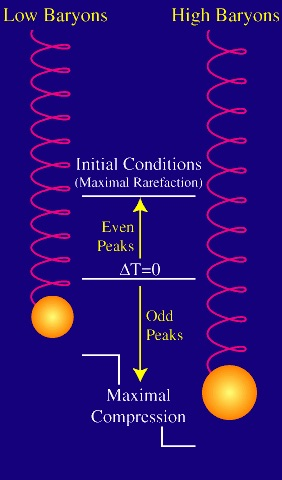
\includegraphics[scale=0.5]{baryonspring}
%\end{figure}
\end{wrapfigure}
Let us consider again the harmonic oscillator model in the case of $\omega_k > \gamma$, small scales where $k$ is big "enough".
The respective solutions are of the form of the damped harmonic oscillator with a shift of $-gm/k$
\[
x = x_0 e^{-\gamma t} e^{\pm i \sqrt{\omega_k ^2 - \gamma ^2} \, t} - \dfrac{g m}{k}
\]
Before recombination, the perturbations of the photon-baryon fluid behaves analogously to the damped harmonic oscillator.\\
During matter dominated era, overdensities of dark matter creates gravitational well where the photon baryon-fluid falls in.
As a consequence the gravitational potential compresses the baryon-photon fluid and the pressure starts to rise.
Since dark matter and baryonic matter are pressureless, the system accretes until the photon pressure causes the fluid to expand outward.\\
The process of compression and expansion gives rise to sound waves and it goes on until recombination.
Only the fluctuations that are caught at the extrema of their oscillations will become peaks in the CMB power spectrum.
Modes caught at the extrema form a harmonic series based on the distance sound can travel by recombination.
The first peak represents the mode that compressed once inside potential wells before recombination, the second the mode that compressed and then rarefied, the third the mode that compressed then rarefied then compressed, etc. exactly as a spring!
The radiation pressure acts as a spring, whereas the inertia of the fluid as the mass of the ball.\\
The temperature fluctuations are damped due to collisions between the baryons and the photons that dissipate energy, and the expansion of the universe.\\
%The damping scale provides another standard ruler for the curvature test
The physical scale of the damping depends on the baryon density through the mean free path
%And the matter density through the time available for the photons to random walk.

\begin{comment}
If we can calibrate the distance CMB photons random walk during recombination, we have another standard ruler for the angular diameter distance test of the spatial curvature of the universe.  Remember that we measure its angular scale in the power spectrum itself.

Alternatively, if we know the curvature of the universe we can infer the physical distance the photons travel.  In the standard model, the physical distance depends only on the baryon density and the dark matter density (matter-radiation ratio).  Since all three (curvature, baryons density and matter radiation) are measured by the positions and heights of the peaks themselves, the damping tail provides a beautiful consistency test for the standard model.

Let's see how that works.

Microphysically, the distance photons can travel is related to a random walk process.  Remember that the photons have a certain mean free path in the baryons defined as the average distance the photon travels before Thomson scattering off a free electron:\\
Raising the number of baryons, decreases the mean free path and hence shortens the distance photons can travel at recombination.  Finally the full distance also depends on the amount of time the photons have to random walk and hence the age of the universe at recombination.  Remember that the age is determined by the dark matter density.  Mathematically, the length is roughly the geometric mean of the mean free path and the distance light can travel without obstruction (the horizon scale).
%
%
%
%
    This text will not be displayed.

 by starting from the continuity and Euler equation for a photon fluid with  number density $n$, energy density $u$ and pressure $p$:
\begin{equation}
\label{hydro}
\dot{n} + n_0 \vec{\nabla} \cdot \vec{v} = 0 \qquad
\dot{\vec{v}} = - c^2 \dfrac{\vec{\nabla} \delta p}{p_0 + u_0} - \vec{\nabla} \delta \Phi
\end{equation}
where $v$ is the streaming velocity of the perturbations and the subscript $_0$ indicates the background average values of th correspondent quantities.\\

So, the temperature fluctuations are related to the number density, energy density and pressure as follow:
\begin{equation}
\dfrac{\delta n}{n_0} = 3 \Theta \qquad
\dfrac{\delta u}{u_0} = 4 \Theta = \dfrac{\delta p}{p_0}
\end{equation}
We can rewrite eq.(\ref{hydro}) in terms of the temperature fluctuations:
\begin{equation}
\dot{\Theta} + \nabla \cdot \vec{v} = 0 \qquad \dot{\vec{v}} = - c^2 \vec{\nabla} \Theta - \vec{\nabla} \delta \Phi
\end{equation}
where we used $p_0 + u_0 = 4 p_0$

\begin{itemize}
\item hydrodynamics \citep{huLectureNotesCMB2008}
page 14 eq 49 to page 17 eq 71\\
skip doppler effect
\item gravito acoustic oscillations page 19 up to eq 82 , justify briefly constant potential in page 20
% if stress perturbations are negligible compared with density perturbations ( δp ≪ δρ ) then the potential will remain constant in periods where the background equation of state p/ρ is constant
\item page 20 and 21 up to eq92 important comment 
%The consequence is that overdense regions where Ψ is negative (potential wells) are cold spots in the effective temperature.
\item baryonic effect
\end{itemize}
\end{comment}


\section{Comments on the results and plots of the CMB spectrum}
We have outlined how we expect matter to behave at large and small scales.
Let us now see if our predictions are compatible with the measured temperature power spectrum.
The behavior of the primordial plasma is imprinted in the CMB photons, in fact, we observe the density fluctuations as anisotropies in the sky map tempearature.
In order to relate the fluctuations at different scales and the deviations from the average temperature $2.7$ K on the CMB map, it is necessary to decompose the observed temperature deviation $T(\theta, \phi)$ into a set of orthonormal functions on the sky.
The spherical harmonics $Y^{m} _{l} (\theta, \phi)$ are suitable for this.\\
So if $T(\theta,\phi)$ is the temperature at position $(\theta,\phi)$ on the sky map,
we can write:
\begin{equation}
T(\theta, \phi) = \sum _{l, m} a_{lm} Y^{m} _l (\theta, \phi)
\end{equation}
Due to the orthonormality of the spherical harmonics, we obtain the coeaficients:
\begin{equation}
a_{lm} = \int _0 ^{2 \pi} \dd \phi \int _0  ^{\pi} \dd \theta \,
\sin( \theta) \, T(\theta, \phi) \, Y^{m} _l (\theta, \phi)
 \end{equation}
We define the power spectrum of the temperature map as 
 \begin{equation}
 C_l = \dfrac{1}{2l+1} \sum _{m=-l} ^{l} |a_{lm}|^2
 \end{equation}
Since $l \sim 1/ \theta$, for small $l$ we are considering big scales of the sky map, viceversa for big $l$.
As we consider increasing $l$ we are looking at fluctuations in the primordial plasma that have a decreasing  scale and thus a smaller wavelength.\\
The measured temperature power spectrum is shown in Figure(\ref{temp_pow_spect}).
%
%
%
\begin{figure}
\centering
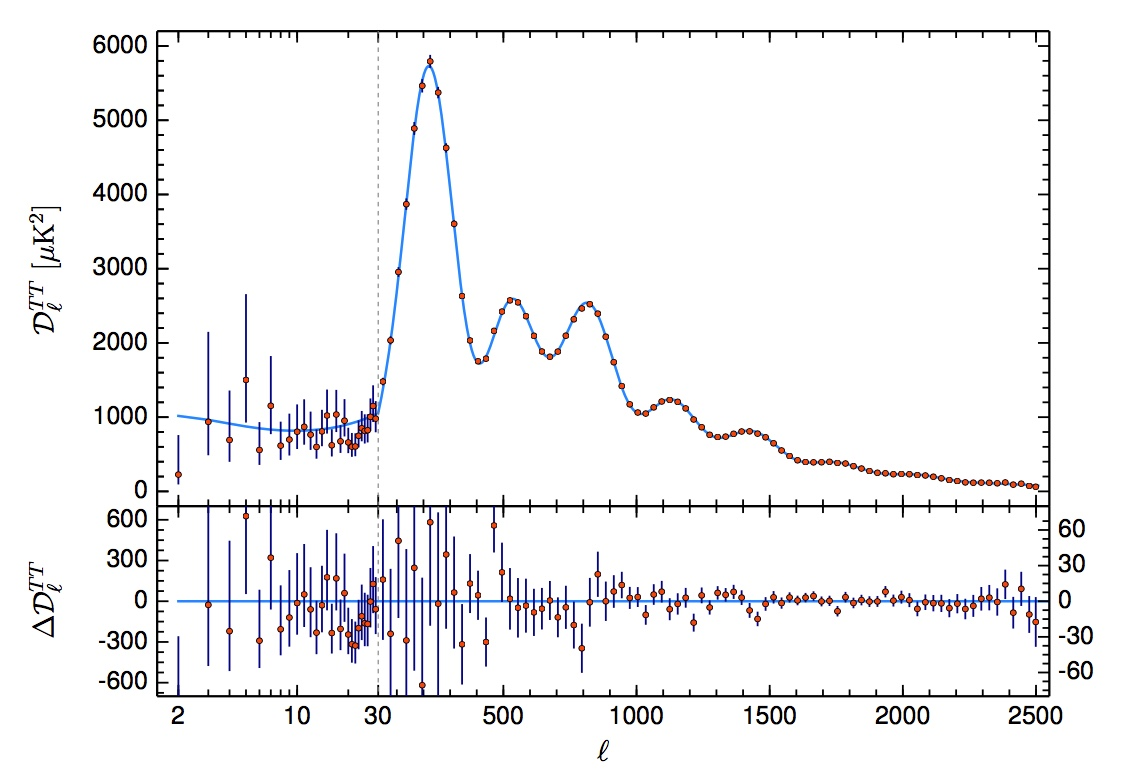
\includegraphics[width=0.9\textwidth]{planck2018}
\caption{Planck 2018 temperature power spectrum. $\mathcal{D}^{TT}_l = l(l+1)C_l$ (arXiv:1807.06209v1)}
\label{temp_pow_spect}
\end{figure}
%
%
%
For large scales, small $l<30$, the power spectrum is constant and oscillations do not take place.
Therefore, the Sachs-Wolfe effect is dominant on large scales where the oscillations have too large wavelength to complete an entire oscillations before recombination and they experience mainly the gravitational redshift.\\
For large $l$ the acoustic oscillations are dominant.
The first peak is at $l \approx 200$ approximately $1 ^o$ on the sky, it represents how the tiny variations in the fluid density gave rise to a sound wave which collapsed exactly at the time of recombination.
The position of the peak tells us at which scale the first total compression of the primordial plasma happened.
The second peak is linked to those oscillations that compressed and expanded, and they reached the maximal rarefaction of the plasma at recombinatio.
The third peak is related to the oscillations that collapsed expanded and recollapsed, and so on for the higher peaks.\\
Notice that as we consider higher and higher $l$, i.e. smaller scales, the damping effects become relevant, especially for  $l>10^{3}$.\\

The four density parameters $\Omega$ encode the energy-matter content of the Universe and they determine the evolution of space-time through the Friedmann equations. 
We want now to link the information contained in the measured fluctuations of the CMB to the density parameters through the observed power spectrum.\\


\subsection{Dark Energy and Curvature}
The cosmological constant $\Lambda$ was introduced in the Einstein's field equations as a possible parameter of our cosmological model.
It turns out from the measurements of the Hubble constant $H_0$ and distant supernovae that the Universe is not only expanding but accelerating.
Therefore, from the Friedmann equations we know that the cosmological constant plays a crucial role in the expansion and in the future evolution of the Universe.
This mysterious energy that leads to the expansion of the Univers is called Dark Energy.\\
Form Figure(\ref{DE_curv} b) we can notice that the dark energy density $\Omega_{\Lambda0}$ plays a small role in the position of the peaks. 
In fact, the  cosmological constant produces a small change in the distance light can travel since recombination and this influences the scale at which we measure the peaks.\\
The position of the peaks is instead particularly sensitive to the cruvature of the Universe, as show in Figure(\ref{DE_curv}a).
The curvature determines how anlges are deformed.
By measuring the position of the first peak we know the angle $\theta \sim 1/l$ of the oscillations.
If I multiply by the angle by the distance (specifically the angular distance) I obtain the size of the oscillations for Euclidean geometry $k =0$.
The first peak represents the first complete compression of the photon-bryon fluid, so by multplying the sound speed of the fluid times the time of the collapse times the expansion factor I obtain the size of the oscillations and I can compare it with the estimated size in order to check the curvature parameter.
	TO BE EXPLAINED DECENTLY




% Given our current uncertainties about the physical density of the matter, the distance that sound can travel by recombination is currently uncertain, a fact related to the matter's effect on the age of the universe at recombination.  Likewise we have assumed that the physical density of the baryons  (Omegabh2) is fixed.  Baryons lower the speed of sound in the medium and hence also affect the distance sound can travel.  Luckily both of these quantities dramatically change the shape of the peaks as we shall see.  They will be measured once the higher peaks are detected and will no longer confuse the measurement of the curvature.   As it turns out, the sound horizon is not a standard ruler but rather a standardizeable ruler.
\begin{figure}
\begin{center}
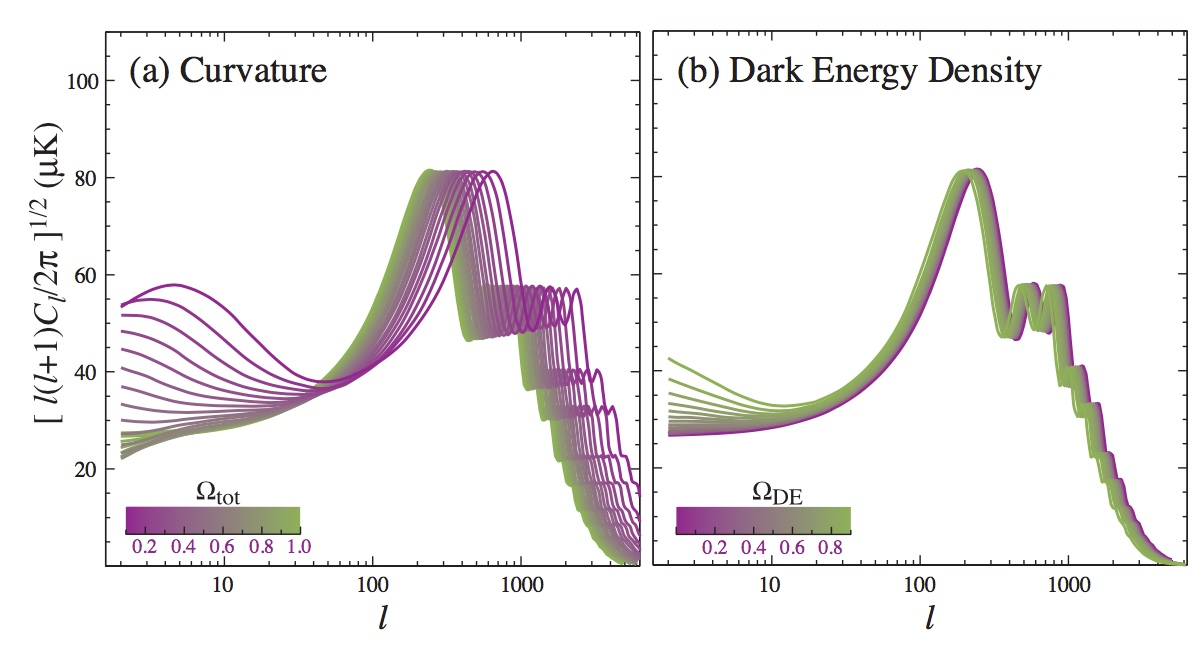
\includegraphics[width=\textwidth]{curvature_de}
\end{center}
\caption{}
\label{DE_curv}
\end{figure}

\subsection{Dark Matter and Baryons}
Baryons (or ordinary matter) load down the photon-baryon plasma and add inertial (and gravitational) mass to the oscillating system.

Their effect on the acoustic peaks is easy to understand.  Remember what happens when you add mass to a spring and let it fall in the gravitational field of the Earth.  With more mass loading the spring, it falls further before pulled back by the spring.  On the other hand, it rebounds to the same position it started from. 

Since the odd numbered (first, third, fifth...) acoustic peaks are associated with how far the plasma "falls" into gravitational potential wells (how much the plasma compresses), they are enhanced by an increase in the amount of baryons in the universe.   The even numbered peaks (second, fourth, sixth) are associated with how far the plasma "rebounds" (how much the plasma rarefies).  Thus with the addition of baryons the odd peaks are enhanced over the even peaks.  For example, baryons make the first acoustic peak much larger than the second.  The more baryons the more the second peak is relatively suppressed. 
\par

%http://background.uchicago.edu/~whu/intermediate/baryons2.html
\paragraph{image}
Power spectrum shows baryons enhance every other peak.
Second peak is suppressed compared with the first and third
Additional effects on the peak position and damping yield consistency checks
When we do the full calculation of the power spectrum, the basic physics of a mass on the spring appears as advertised.   The odd numbered acoustic peaks in the power spectrum are enhanced in amplitude over the even numbered ones as we increase the baryon density of the universe.\\
Note: Cosmologists label the baryon density in terms of its fraction of the critical density Wbtimes the Hubble constant squared (in units of 100 km/s/Mpc) to get something proportional to the physical density of the baryons.]

There are two other related effects due to the baryons:  since adding mass to a spring slows the oscillation down, adding baryons to the plasma decrease the frequency of the oscillations pushing the position of the peaks to slightly higher multipoles l.

Baryons also affect the way the sound waves damp and hence how the power spectrum falls off at high multipole moment lor small angular scales as we will see later.

The many ways that baryons show up in the power spectrum imply that the power spectrum has many independent checks on the baryon density of the universe.  The baryon density is a quantity that the CMB can measure to exquisite precision.

\paragraph{dark matter}
Second peak is observed to be substantially lower than first peak
Dark baryons of at least the big-bang nucleosynethesis density required
Although we cannot yet claim that the second peak is as precisely measured as the first, we can say that (assuming it exists!) it is definitely of lower amplitude than the first:\\
The current data indicate that the baryon density is around Omegabh2=0.02 This value is interesting since it is also the baryon density inferred from the abundance of deuterium at high redshift in quasar absorption lines and the theory of big-bang nucleosynthesis.  We now have an additional and independent line of evidence that there are missing baryons in the universe - i.e. that most the baryons are not in stars.   Once the second and higher peaks are definitively measured, CMB constraints on the baryon density will sharpen considerably (ultimately to a few percent accuracy).  Needless to say it will be interesting to see how these comparisons shape up as the data improve.
\paragraph{dark}
Raising the dark matter density reduces the overall amplitude of the peaks.
Lowering the dark matter density eliminates the baryon loading effect so that a high third peak is an indication of dark matter.
With three peaks, its effects are distinct from the baryons
Measuring the dark matter density resolves the main ambiguity in the curvature measurement
As advertised the acoustic peaks in the power spectrum are sensitive to the dark matter density in the universe.  (Formally, the matter to radiation ratio but the radiation density is fixed in the standard model.)\\
As we raise the physical density of the dark matter, Wmh2, the driving effect goes away at a given peak such that its amplitude decreases.  Although this effect changes the heights of all the peaks, it is only separable from the baryonic effects with at least three peaks.  Note that decreasing the matter density also affects the baryon loading since the dark matter potential wells go away leaving nothing for the baryons to fall into. Having a third peak that is boosted to a height comparable to or exceeding the second peak is an indication that dark matter dominated the matter density in the plasma before recombination. Note that the self-gravity of the photons and baryons still plays a role in the first and second peaks so that the third peak is the cleanest test of this behavior.

Notice also that the location of the peaks, and that of the first peak in particular, changes as we change the dark matter density.  The matter to radiation ratio also controls the age of the universe at recombination and hence how far sound can travel relative to how far light travels after recombination.  This is the leading order ambiguity in the measurement of the spatial curvature of the universe.  We see here that that ambiguity will be resolved when at least three peaks are precisely measured.





\begin{figure}
\begin{center}
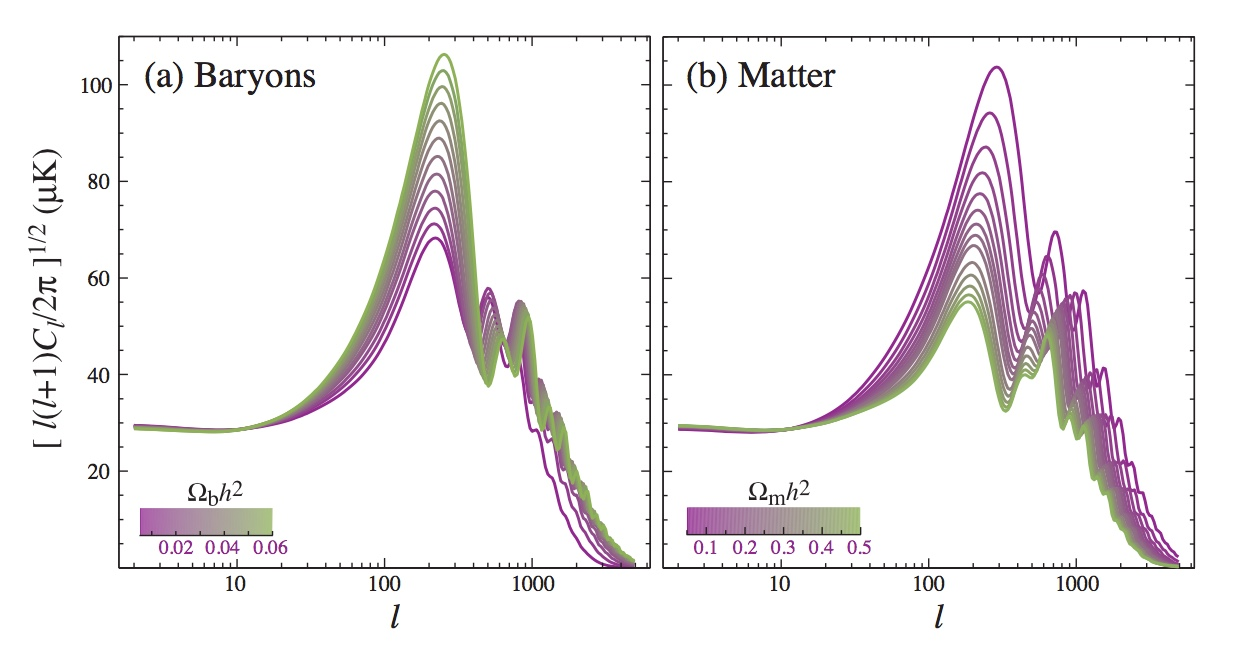
\includegraphics[width=\textwidth]{baryon_m}
\caption{aa}
\end{center}
\label{DM_bar}
\end{figure}
\section{Conclusion}
nn
\citep{padmanabhanDetectingDarkMatter2005}



\bibliographystyle{plain}
\bibliography{dark_1}
\end{document}
